\section{Data visualization}

\subsection{Definition}
A number of definitions have been attributed to explain what data visualization means. According to Friendly \cite{Friendly2009} the term arose together with the birth of statistical thinking, being a way to illustrate mathematical language, their trends, tendencies and distributions trough the use of diagrams and graphics. Few \cite{StephenFew2013} describes it as a graphical display of abstract information for the purpose of sense-making and communication. However, for the grounds of my project, the term can be  ambiguous without bearing in mind the last decade advances in statistics and computer science, in the sense that the aforementioned concepts do not exclude printed or non-computerized data representations like the shown in figure \ref{fig:air_pollution_infographic}. Thus, the definition offered by Iliinsky and Steele \cite{Iliinsky2011} is more specific: 
\begin{displayquote}
Any visual representation of data that is:
	\begin{itemize}
	\item algorithmically drawn (may have custom touches but is largely rendered with the help of computerized methods);
	\item easy to regenerate with different data (the same form may be repurposed to represent different datasets with similar dimensions or characteristics);
	\item often aesthetically barren (data is not decorated); and
	\item relatively data-rich (large volumes of data are welcome and viable, in contrast to infographics).
    \end{itemize}
\end{displayquote}

\begin{figure}[h]
  \centering
  \begin{adjustbox}{width=.8\textwidth,center=\textwidth}
  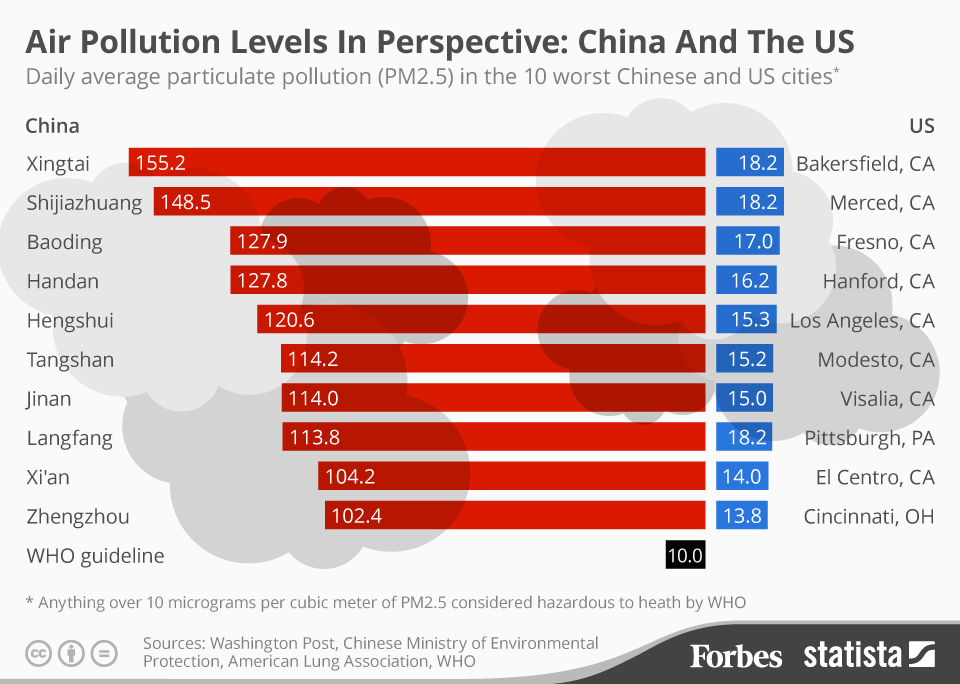
\includegraphics[scale=1]{images/air_pollution_infographic.jpg}
  \end{adjustbox}
  \caption[Air pollution infographic]{Air pollution infographic \cite{NiallMcCarthy}}
  \label{fig:air_pollution_infographic}
\end{figure}

A visualization helps towards understanding data  by taking advantage of the human visual system to process a large amount of information quickly, thus allowing the human brain to identify patterns, links and relationships between the represented objects. Daniel et al. \cite{KeimDaniel2010}, also states that visualizing enables people to: 
\begin{displayquote}
	\begin{itemize}
\item  Synthesise information and derive insight from massive, dynamic, ambigu- ous, and often conflicting data.
\item Detect the expected and discover the unexpected.
\item Provide timely, defensible, and understandable assessments.
\item Communicate these assessment effectively for action.
	\end{itemize}
\end{displayquote}

Data visualization is essential when the available data is vast and dynamic, and when raw data does not make sense by its own. Therefore, data must be encoded using technological, and design elements;  potentially making use of disciplines such as statics, data mining, human computer interaction and graphic design. 

\subsection{Designing data visualizations}
The figure in \ref{fig:data_visualization_process} depicts the visual analysis process according Daniel et al. \cite{KeimDaniel2010}. In the first stage,  data should be collected, (usually from many distinct data sources) and standardized into one common format. This later enables to choose between the creation of models, or visualizations; models are an automated representation that requires data mining techniques; whereas visualizations are manual representations that can be created through simple mapping from data to the visual context. Both representations are linked together, to enable validation and refinement through iteration. The final stage; which is the one we are more concerned with; is the knowledge gained from the representation; which will aim to respond the questions for which they were created in the first place.
\begin{figure}[!htb]
\begin{adjustbox}{width=1\textwidth,center=\textwidth}
  \centering
  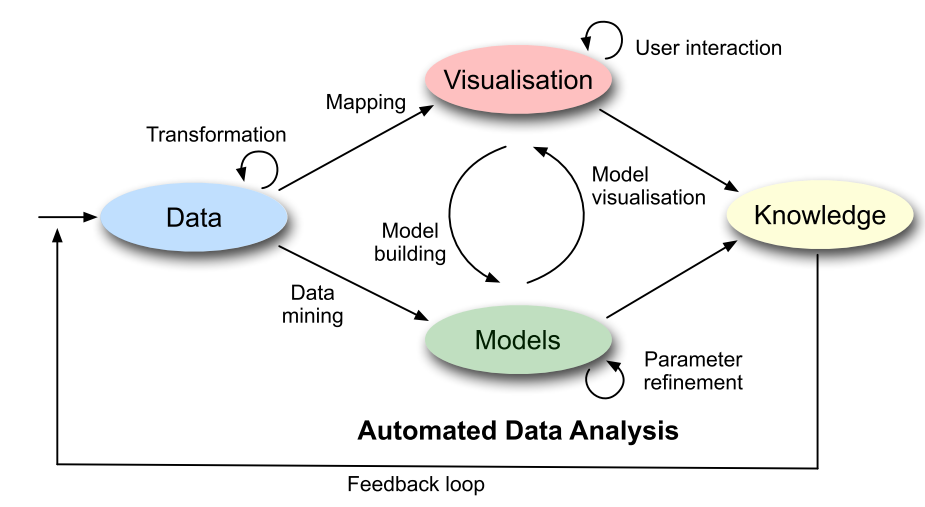
\includegraphics[scale=1]{images/data_visualization_process.png}
\end{adjustbox}
  \caption[The data visualization process \cite{KeimDaniel2010} ]{The data visualization process \cite{KeimDaniel2010} }
  \label{fig:data_visualization_process}
\end{figure}

According to Ben Fry \cite{Cleveland1993}, one specific approach for data visualizations is illustrated in figure \ref{fig:data_visualization_stages}, which establishes a common series of steps that can be followed for this purpose :

\begin{displayquote}
	\begin{itemize}
\item Acquire: Obtain the data, whether from a file on a disk or a source over a network. 
\item Parse: Provide some structure for the data’s meaning, and order it into categories. 
\item Filter: Remove all but the data of interest. 
\item Mine: Apply methods from statistics or data mining as a way to discern patterns or place the data in mathematical context.
\item Represent: Choose a basic visual model, such as a bar graph, list, or tree. 
\item Refine: Improve the basic representation to make it clearer and more visually engaging. 
\item Interact: Add methods for manipulating the data or controlling what features are visible.
\end{itemize}
\end{displayquote}

\begin{figure}[!htb]
\begin{adjustbox}{width=1\textwidth,center=\textwidth}
  \centering
  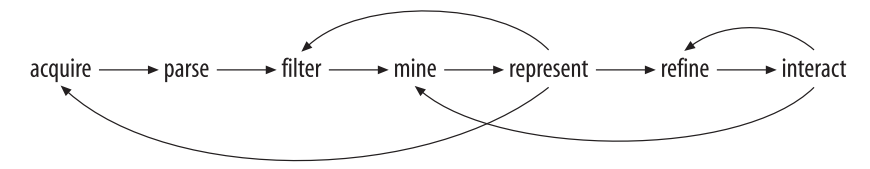
\includegraphics[scale=1]{images/visualization_stages.png}
\end{adjustbox}
  \caption[Visualization stages \cite{Cleveland1993} ]{Visualization stages  \cite{Cleveland1993} }
  \label{fig:data_visualization_stages}
\end{figure}
These visualization stages start again from a question, which may not be immediate answerable from the raw data, and goes through the steps until arriving a desired answer; it is also observed that the stages are linked together and one may back to redefine the process at some stage. Both methods mentioned above s are similar in between. While the later builds an easy to follow framework for any visualization project; the former recognizes that not all steps are needed in many situations.

\subsection{Data visualizations for decision support}
"A decision-making process usually includes the acquisition of related information, the construction of a mental representation of the problem and solutions, and the identification of an optimal solution" \cite{carroll1987mental} as cited in \cite{Zhu2008}, decision making involves acquiring domain specific information about a particular question; which is the intended output of a data visualization. It is therefore important to understand the effects of data visualizations in decision support making, if any.

The decision making process takes into account the decision maker's skill, the decision task, and the problem space. In our specific context, the decision maker, should be able to understand the data in its represented space (visualization), evaluate the problem (avoid air pollution), and execute a decision task (leave the polluted space). "A well designed visualization takes features of the decision task and the characteristics of the decision makers into consideration" \cite{Zhu2008}. Thus, visualizations should be created in the specific context of the decision makers; discovering beforehand the knowledge they should have; the problems they are likely to face; and the potential decisions they should be able to take. 
